% This file was created with tikzplotlib v0.10.1.post5.
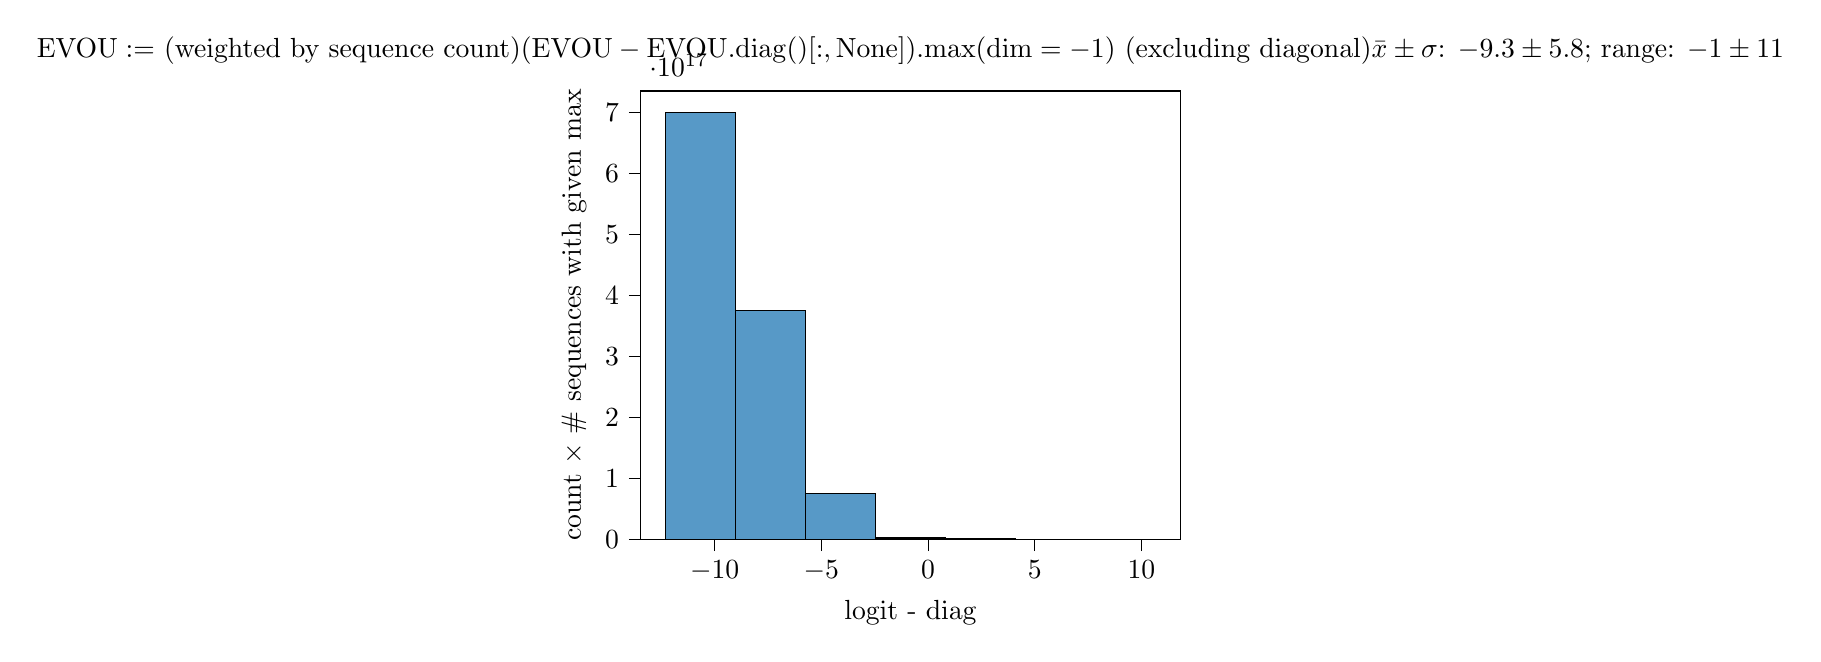
\begin{tikzpicture}

\definecolor{darkgray176}{RGB}{176,176,176}
\definecolor{steelblue31119180}{RGB}{31,119,180}

\begin{axis}[
tick align=outside,
tick pos=left,
title={\(\displaystyle \mathrm{EVOU} := \WE \WV \WO\WU \) (weighted by sequence count)\\
\(\displaystyle (\mathrm{EVOU} - \mathrm{EVOU}\mathrm{.diag}()[:,\mathrm{None}])\mathrm{.max}(\mathrm{dim}=-1)\) (excluding diagonal)\\
\(\displaystyle \bar{x}\pm\sigma\): \(\displaystyle -9.3 \pm 5.8\); range: \(\displaystyle -1 \pm 11\)},
x grid style={darkgray176},
xlabel={logit - diag},
xmin=-13.466238117218, xmax=11.8224678993225,
xtick style={color=black},
xtick={-15,-10,-5,0,5,10,15},
xticklabels={
  \(\displaystyle {\ensuremath{-}15}\),
  \(\displaystyle {\ensuremath{-}10}\),
  \(\displaystyle {\ensuremath{-}5}\),
  \(\displaystyle {0}\),
  \(\displaystyle {5}\),
  \(\displaystyle {10}\),
  \(\displaystyle {15}\)
},
y grid style={darkgray176},
ylabel={count \ensuremath{\times} \# sequences with given max},
ymin=0, ymax=7.35559223350332e+17,
ytick style={color=black},
ytick={0,1e+17,2e+17,3e+17,4e+17,5e+17,6e+17,7e+17,8e+17},
yticklabels={
  \(\displaystyle {0}\),
  \(\displaystyle {1}\),
  \(\displaystyle {2}\),
  \(\displaystyle {3}\),
  \(\displaystyle {4}\),
  \(\displaystyle {5}\),
  \(\displaystyle {6}\),
  \(\displaystyle {7}\),
  \(\displaystyle {8}\)
}
]
\draw[draw=black,fill=steelblue31119180,fill opacity=0.75] (axis cs:-12.3167514801025,0) rectangle (axis cs:-9.03250394548689,7.00532593666983e+17);
\draw[draw=black,fill=steelblue31119180,fill opacity=0.75] (axis cs:-9.03250394548689,0) rectangle (axis cs:-5.74825641087123,3.75185743754065e+17);
\draw[draw=black,fill=steelblue31119180,fill opacity=0.75] (axis cs:-5.74825641087123,0) rectangle (axis cs:-2.46400887625558,7.44446198322835e+16);
\draw[draw=black,fill=steelblue31119180,fill opacity=0.75] (axis cs:-2.46400887625558,0) rectangle (axis cs:0.820238658360072,2.16805735351562e+15);
\draw[draw=black,fill=steelblue31119180,fill opacity=0.75] (axis cs:0.820238658360072,0) rectangle (axis cs:4.10448619297572,436780984433849);
\draw[draw=black,fill=steelblue31119180,fill opacity=0.75] (axis cs:4.10448619297572,0) rectangle (axis cs:7.38873372759138,151191815363248);
\draw[draw=black,fill=steelblue31119180,fill opacity=0.75] (axis cs:7.38873372759138,0) rectangle (axis cs:10.672981262207,2517200202903);
\end{axis}

\end{tikzpicture}
